Pour le second semestre, l'approche retenue est l'apprentissage par renforcement (\textit{Reinforcement Learning}) afin d'automatiser les décisions de placement et d'autoscaling. L'agent apprend à piloter simultanément le \textbf{nombre de pods} alloués à chaque fonction et leur \textbf{placement} sur les nœuds du cluster, en optimisant le compromis énergie/latence.

L'environnement de simulation \textit{Smart City} (FaaS-Sim) est traduit en interface standardisée \texttt{gymnasium}~\cite{brockman2016gym}. Le simulateur est discrétisé : toutes les $X$ secondes (\texttt{step\_duration}), l'agent observe l'état courant — latence moyenne des dernières requêtes et nombre de pods (\texttt{replicas}) actifs par fonction — puis émet une action de \textit{scaling}. L'espace d'action est un vecteur \texttt{MultiDiscrete} (valeurs de 0 à 16 par fonction) ; la transformation $action - 8$ produit un ordre allant de $-8$ pods (scale-down) à $+8$ pods (scale-up).

L'algorithme \textbf{PPO} (\textit{Proximal Policy Optimization})~\cite{schulman2017ppo} a été retenu car il est particulièrement adapté aux espaces d'actions discrètes multiples (6 fonctions indépendantes). Un suivi via \textbf{TensorBoard} permet d'observer les métriques internes du réseau (\textit{Value Loss}, entropie) et les métriques de simulation (SLA, consommation électrique) afin de valider la stabilité de l'apprentissage.
\begin{figure}[htbp]
    \centering
    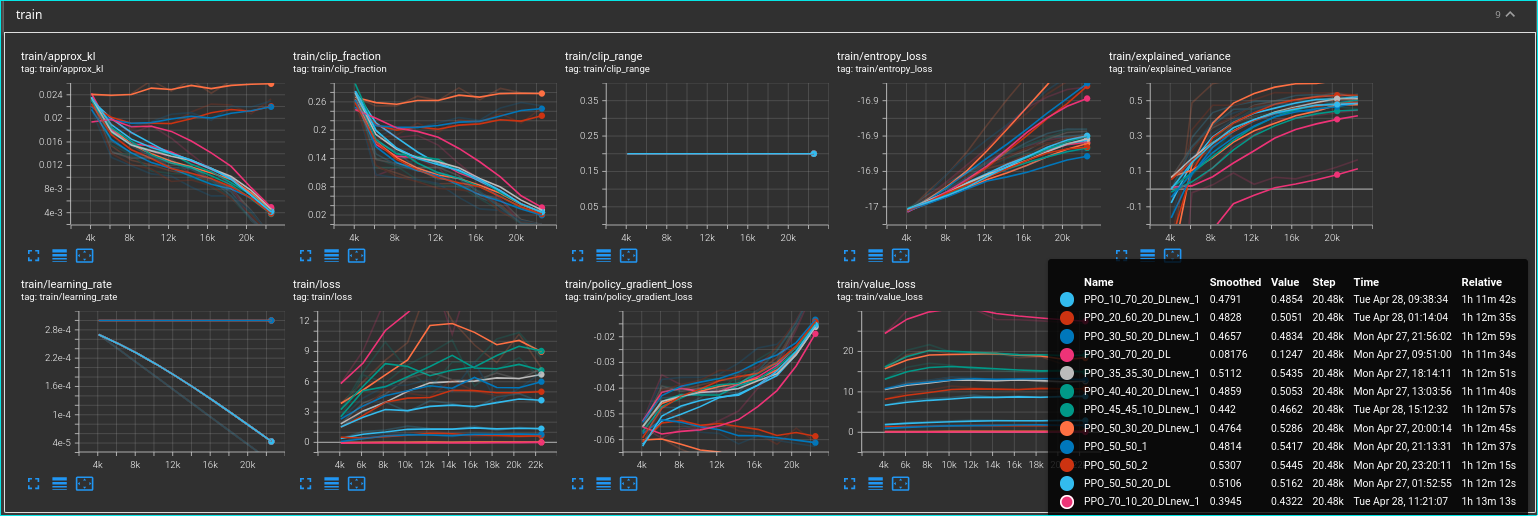
\includegraphics[width=0.72\textwidth]{images/tensorboard.png}
    \caption{Monitoring TensorBoard : évolution des métriques d'apprentissage PPO}
    \label{fig:tensorboard}
\end{figure}

Le taux d'apprentissage (\texttt{learning\_rate}) décroît linéairement jusqu'à 0 en fin d'entraînement pour préserver les politiques optimisées acquises.

La fonction de récompense normalise chaque métrique brute en un score dans $[0,1]$ pour rendre les unités comparables (les secondes du SLA et les Watts de l'énergie n'étant pas directement comparables) :
$$Reward = (\alpha \times \underbrace{SLA}_{\text{taux de respect}}) + (\beta \times \underbrace{Energy}_{\text{éco. norm.}}) + (\gamma \times \underbrace{Efficiency}_{\text{req./pods actifs}})$$
avec $\alpha + \beta + \gamma = 1$, bornant le score maximal à 1,0. Le terme $Efficiency = \frac{\text{Requêtes}}{\text{Pods Actifs}}$ pénalise le sur-provisionnement (\textit{over-provisioning}) : allouer des pods inutilisés est directement puni. L'énergie maximale de référence est verrouillée sur l'inventaire physique total du cluster, empêchant l'agent de tricher en allumant des nœuds pour gonfler artificiellement ce maximum.
